%%%%%%%%%%%%%%%%%%%%%%%%%%%%%%%%%%%%%%%%%%%%%%%%%%%%%%%%%%%%%%%%%%
\subsubsection{Radial--torsional ring [PROPOSED]}\label{sec:rotational}
%%%%%%%%%%%%%%%%%%%%%%%%%%%%%%%%%%%%%%%%%%%%%%%%%%%%%%%%%%%%%%%%%%
% Data behind every table and figure of this subsubsection are the small derived files
% paper-data/rotational_{convergence,mixed_terms,acceptance_counts,floor_by_qoi,order_intervals}.csv;
% figures/rotational_convergence.pdf and figures/rotational_mixed_terms.pdf plot the first two.

\todo{STATUS: the benchmark is \emph{proposed} for category A; the combined member is not category A while the origin of its reference-error floor is open and no independent nonlinear check of the reference exists. Items still missing for category A: member-specific self-convergence studies of the CFD solutions to the reference limit, a pinned reproducibility kit (case files, reference scripts, versions, hashes, archived with a persistent identifier) and an explicit ``planar, rotationally invariant ($n=0$) branch'' statement in the case documentation. The solids4foam tutorial is being prepared separately. The cited prior-art references were checked against Crossref metadata only; their content statements rest on a literature review (full text for the Wang--Pironneau preprint version, Serino et al.\ and Hessenthaler et al.; the published Wang--Pironneau version and Polignone--Horgan not read in full) and must be re-read before submission. The LaTeX build of this section has not been verified.}

\paragraph{What it tests.}
Both category-A cases of Section~\ref{sec:exact_refs} exercise the radial response of a linear, small-amplitude wall (added mass in ringAddedMass; wave propagation and radial traction in womersleyTube) and carry no rotational degree of freedom.
The radial--torsional ring adds three features that they cannot test.
(i)~A swirl (azimuthal) velocity of the fluid, whose angular momentum is transported by diffusion and, with a radial through-flow, by convection on a moving domain; the interface transmits a tangential traction (torque) rather than only a normal one.
(ii)~Interface rotation and tangential mesh motion, which enter the Piola traction map and the wall velocity.
(iii)~A nonlinear stretch--rotation coupling: in a finite-strain, compressible solid a finite twist forces a radial deformation of order $\theta^2$, and the solid carries its own centripetal and Coriolis accelerations, none of which exist in a linear radial or torsion-only model.
The first two are rotational counterparts of the added-mass and traction transfer tested elsewhere in the suite; the third is a finite-amplitude interaction that only a combined radial and rotational loading reveals.
The problem is planar and rotationally invariant (an in-plane rotation of an annulus, not axial swirl in a tube), so that a two-dimensional OpenFOAM case is sufficient and no wedge mesh is required.

\paragraph{Definition.}
A neo-Hookean (compressible) solid annulus $0.5\le R\le1\,\mathrm{m}$ (plane strain, $\rho_S=1000\,\mathrm{kg/m^3}$, $E_S=2\times10^4\,\mathrm{Pa}$, $\nu_S=0.3$) surrounds the fluid region $b(t)\le r\le c=2\,\mathrm{m}$ ($\rho_F=1000\,\mathrm{kg/m^3}$, $\mu_F=300\,\mathrm{Pa\,s}$), $b(t)$ being the deformed interface radius.
The inner solid boundary is radially clamped and rotated, $\alpha_A=\theta_0 S(t)\sin\Omega t$ with $\Omega=3\,\mathrm{rad/s}$; the outer fluid boundary carries a prescribed pressure $p_c=P_0S(t)$ and a tangentially traction-free open condition.
$S(t)$ is a $C^\infty$ ramp over $T_\mathrm{ramp}=1\,\mathrm{s}$.
Three members are defined by the loading: radial ($P_0=-3\,\mathrm{kPa}$, $\theta_0=0$), torsion ($\theta_0=0.1\,\mathrm{rad}$, $P_0=0$) and combined (both).
The verification below covers $0\le t\le2\,\mathrm{s}$ with $\theta_0=0.1\,\mathrm{rad}$.
Quantities of interest are the interface rotation $\alpha_B$, the wall torque $T_B$ and the shear traction $\sigma_{r\theta}$ at the interface, the drive torque $T_A$, and the solid and fluid angular momenta $H_s$, $H_f$ (all normalised by the maximum of the reference), together with the normal-traction quantities $u_B$, $\sigma_{rr}$ and $p_b$, which are reported but excluded from order claims (see below).

\paragraph{Reference.}
On the planar, rotationally invariant ($n=0$) branch (modes with $n\neq0$ are not part of the reference) the fluid reduces exactly, at any amplitude, to $\mathbf{v}=(Q(t)/r)\,\mathbf{e}_r+w(r,t)\,\mathbf{e}_\theta$, and the solid to a one-dimensional problem in $R$ with the radial displacement $\varphi(R,t)$ and the rotation $\alpha(R,t)$.
The coupled finite-amplitude problem is thereby a system of one-dimensional partial differential equations, solved by a spectral space discretisation (GLL, i.e.\ Legendre, modes for the solid and Chebyshev modes for the fluid) and Radau time integration (rtol $10^{-11}$); we call it semi-analytical.
It is not a closed-form solution and its limits are those of the reduced model.
Evidence for the reference, none of which uses solids4foam:
(a)~the reduced equations and the hyperelastic stress of the stated energy were derived and verified symbolically (234 plus 12 exact-arithmetic checks);
(b)~the linear limits reproduce the exact Bessel-function eigenvalues of the torsional and breathing modes to $7\times10^{-13}$ and $2\times10^{-10}$ (relative), and the linear transfer function to $4.5\times10^{-9}$;
(c)~the finite-amplitude static state agrees with an independent boundary-value solution to $10^{-14}$, and the energy and angular-momentum balances close to $2\times10^{-13}$ and $7\times10^{-14}$;
(d)~it is numerically resolved: doubling and tripling the spatial resolution, tightening the tolerances to $10^{-13}$ and changing the integrator (BDF, LSODA) change the maximum of each reference quantity by at most $3.1\times10^{-8}$ ($T_B$, $\sigma_{r\theta}$, combined member) and $\le4\times10^{-10}$ for the rotation and the fluid angular momentum, at least five orders below the CFD errors reported below.
This establishes the numerical accuracy of the reduced model.
It is checked by symbolic derivation, linear Bessel solutions, a static boundary-value problem and conservation closure, not by a second, independent nonlinear implementation, so that the correctness of the finite-amplitude coupled terms rests on the derivation and on these checks.

\paragraph{Evidence.}
The solids4foam calculations use the partitioned solver of Section~\ref{sec:numerical_methods} (IQN-ILS coupling, BDF2, $\Delta t=2.5\,\mathrm{ms}$, \texttt{nNonOrthogonalCorrectors}~2 in the fluid) on three meshes of $n_\theta\times n_{r,s}\times n_{r,f}=64\times8\times16$ (M1), $128\times16\times32$ (M2) and $256\times32\times64$ (M3) cells (azimuthal $\times$ solid radial $\times$ fluid radial), each refined by a factor two.
Every run was a single uninterrupted simulation run from $t=0$ to $2\,\mathrm{s}$ without restart, with all 800 steps accepted (acceptance test below); M1 and M2 ran serially and M3 on four MPI ranks; all families were run at the same time step, so the orders below are spatial at $\Delta t=2.5\,\mathrm{ms}$ and no temporal order is claimed.
Two features of the set-up should be stated.
First, with \texttt{nNonOrthogonalCorrectors}~0 the fluid PIMPLE outer iteration on M3 loses contractivity near $1.81\,\mathrm{s}$ (the per-pass contraction factor reaches one) and the torsion run fails; with two non-orthogonal correctors the contraction factor of the M3 runs stays at $0.83$--$0.90$ from $1.5\,\mathrm{s}$ and all runs complete.
Halving $\Delta t$ also removed the failure, so the correctors are shown to be sufficient but not necessary, and no unique root cause is claimed.
Second, the outer-iteration absolute tolerance on the interface displacement is $10^{-12}\,\mathrm{m}$ on M1 and M2 but $10^{-10}\,\mathrm{m}$ on M3 ($10^{-12}\,\mathrm{m}$ stalled on M3); this affects the 31--77 steps accepted by the absolute criterion in the start-up ramp ($t\lesssim0.35\,\mathrm{s}$; torsion 68, 70, 77 and combined 31, 32, 65 on M1, M2, M3, by the verification driver's per-step definition), and its effect was quantified on M2 only (see below).

\emph{Coupling acceptance test.}
A coupling step is accepted when either relative residual measure of Eq.~\eqref{eq:coupling_residuals} is below the tolerance $10^{-6}$ (\texttt{requireAllResidualMeasures} unset, i.e.\ the legacy minimum test) or the absolute interface point mismatch is below the absolute tolerance.
Table~\ref{tab:rot_accept} lists how each step was accepted.
At acceptance the median $r_1$ is $4\times10^{-5}$--$10^{-4}$ and its maximum $1.0$--$1.5\times10^{-2}$, and the absolute point mismatch is $\le4.8\times10^{-7}\,\mathrm{m}$.
Most steps are therefore accepted on $r_2$ alone: only $17$--$56$ of the 800 steps of any run meet both relative measures.
Two different percentages are used and kept apart.
(A) The percentage of steps that fail a test requiring both relative measures below $10^{-6}$ (absolute-tolerance acceptances count as failing), the column ``A'' of Table~\ref{tab:rot_accept}: $93.0$--$97.5\%$ for the six torsion and combined runs ($97.9\%$ for the M2 combined run with absolute tolerance $10^{-10}\,\mathrm{m}$, $93.9\%$ for the M1 radial run); this is the test recommended in Section~\ref{sec:convergence_method}.
(B) The percentage of steps the solver's own strict mode (\texttt{requireAllResidualMeasures}) would reject, which still accepts steps meeting the absolute tolerance (column ``B''): $82.1$--$92.25\%$ over the eight runs, evaluated at the accepted iterate only.
The share of steps accepted on a single relative measure ($83.4$--$92.9\%$) is a descriptive quantity and is neither A nor B.
The runs are consequently \emph{not} claimed to be converged under either stricter criterion.
The only proxy is a radial-loading run on M2 with the relative tolerance tightened from $10^{-6}$ to $10^{-8}$, which changed $u_B$, $\sigma_{rr}$, $p_b$, interface power and solid kinetic energy by $\le4.3\times10^{-4}$ of $\max|\mathrm{ref}|$; the rotational quantities were not run at a tighter relative tolerance, and are covered only by the numerical-noise estimate reported below ($2.4\times10^{-4}$ torsion, $1.3\times10^{-3}$ combined, of $\max|\mathrm{ref}|$).

\begin{table}[htbp]
	\centering
	\small
	\setlength{\tabcolsep}{4pt}
	\caption{Acceptance of the 800 coupling steps per run (verification driver, per-step definition): both relative measures $\le10^{-6}$; $r_1$ only; $r_2$ only; absolute tolerance only (a predictor-level absolute acceptance followed by an iteration with zero residual is counted as ``both''). Columns A and B: percentage of steps rejected by the both-measures test at $10^{-6}$ (A) and by the solver's strict mode with absolute-tolerance acceptance (B), as defined in the text. Source: \texttt{paper-data/rotational\_acceptance\_counts.csv}.}
	\label{tab:rot_accept}
	\begin{tabular}{llrrrrrr}
		\toprule
		Member & Mesh & both & $r_1$ only & $r_2$ only & absolute & A (\%) & B (\%) \\
		\midrule
		torsion & M1 & 32 & 0 & 700 & 68 & 96.0 & 86.62 \\
		torsion & M2 & 47 & 1 & 682 & 70 & 94.1 & 84.50 \\
		torsion & M3 & 56 & 0 & 667 & 77 & 93.0 & 82.12 \\
		combined & M1 & 26 & 0 & 743 & 31 & 96.8 & 92.25 \\
		combined & M2 & 26 & 0 & 742 & 32 & 96.8 & 92.12 \\
		combined & M3 & 20 & 0 & 715 & 65 & 97.5 & 88.00 \\
		\bottomrule
	\end{tabular}
\end{table}

\emph{Torsion member.}
Table~\ref{tab:rot_torsion} and Fig.~\ref{fig:rot_convergence}a show monotone convergence of all primary rotational quantities towards the reference.
Over the nine primary quantities and the windows $0$--$2$ and $0$--$1.8\,\mathrm{s}$ the observed orders are $1.72$--$2.07$ in the max-norm and $1.71$--$2.04$ in the $L^2$-in-time norm; in Table~\ref{tab:rot_torsion} (max-norm, $0$--$2\,\mathrm{s}$) they are $1.90$--$2.07$ on the M1--M2 and $1.72$--$2.04$ on the M2--M3 pair.
The values outside $1.8$--$2.0$ are $T_A$ (up to $2.07$; $2.02$ over $0$--$1.8\,\mathrm{s}$), the rotation (up to $2.03$, $L^2$), the $L^2$ values $2.01$ of $T_B$ and $\sigma_{r\theta}$ over $0$--$1.8\,\mathrm{s}$, the interface power ($2.01$), the solid kinetic energy (up to $2.04$, after the temporal-error correction) and the fluid angular momentum, which is the lowest at $1.72$ (max-norm; $1.71$ in $L^2$ and $1.68$ after the temporal-error correction) against the reference although its self-difference order is $1.97$; the angular velocity lies at $1.81$--$1.96$ (self-difference order $1.97$).
The M3 errors are $0.08$--$0.2\%$ of the reference maximum.
These orders are consistent with the nominal second order, but are observed from three meshes and do not demonstrate asymptotic convergence.

\begin{table}[htbp]
	\centering
	\small
	\setlength{\tabcolsep}{4pt}
	\caption{Torsion member, three-mesh study at $\Delta t=2.5\,\mathrm{ms}$, \texttt{nNonOrthogonalCorrectors}~2: max-norm error over $0$--$2\,\mathrm{s}$ relative to $\max|\mathrm{ref}|$, observed orders $p_{12}$, $p_{23}$ from the max-norm errors, the range of observed orders over both norms and both time windows (without temporal-error correction), and the interval of $p_{23}$ implied by the numerical noise (first-order propagation, max-norm only; see text). Source: \texttt{paper-data/rotational\_convergence.csv} and \texttt{rotational\_order\_intervals.csv}.}
	\label{tab:rot_torsion}
	\begin{tabular}{lrrrrrcc}
		\toprule
		QoI & M1 & M2 & M3 & $p_{12}$ & $p_{23}$ & $p_{23}$ interval & order range \\
		\midrule
		rotation $\alpha_B$ & $1.17\times10^{-2}$ & $2.97\times10^{-3}$ & $7.56\times10^{-4}$ & 1.98 & 1.98 & 1.97--1.98 & 1.98--2.03 \\
		wall torque $T_B$ & $2.84\times10^{-2}$ & $7.24\times10^{-3}$ & $1.89\times10^{-3}$ & 1.97 & 1.94 & 1.75--2.12 & 1.85--2.01 \\
		shear traction $\sigma_{r\theta}$ & $2.76\times10^{-2}$ & $7.04\times10^{-3}$ & $1.86\times10^{-3}$ & 1.97 & 1.92 & 1.73--2.11 & 1.83--2.01 \\
		drive torque $T_A$ & $2.83\times10^{-2}$ & $6.75\times10^{-3}$ & $1.64\times10^{-3}$ & 2.07 & 2.04 & 1.82--2.25 & 1.99--2.07 \\
		solid ang.\ momentum $H_s$ & $1.75\times10^{-2}$ & $4.51\times10^{-3}$ & $1.17\times10^{-3}$ & 1.95 & 1.95 & 1.64--2.26 & 1.89--1.97 \\
		fluid ang.\ momentum $H_f$ & $2.19\times10^{-2}$ & $5.86\times10^{-3}$ & $1.78\times10^{-3}$ & 1.90 & 1.72 & 1.72 & 1.71--1.91 \\
		\bottomrule
	\end{tabular}
\end{table}

The following limit these statements.
The temporal error at $\Delta t=2.5\,\mathrm{ms}$ was estimated from a fixed-mesh pair at half the time step on M2 (Richardson extrapolation assuming order two, not measured) and amounts to $5$--$25\%$ of the M3 error (torque, shear traction and interface power $20$--$25\%$); correcting for it lowers the torque orders on the M2--M3 pair to 1.86--1.88.
The error at fixed $\Delta t$ extrapolated from the finest pair is $13$--$47\%$ of the M3 error, so floors are visible.
The max-norm errors of the torque-type quantities carry numerical (partitioning and iteration) noise of about $2.4\times10^{-4}$ of $\max|\mathrm{ref}|$ in the torsion runs and about $1.3\times10^{-3}$ in the combined runs (torque $1.26\times10^{-3}$, shear traction $1.21\times10^{-3}$, drive torque $8.9\times10^{-4}$), estimated from comparisons of serial and four-rank runs and of coupling tolerances on M2; for the rotation and the angular momenta of the combined runs it is $\lesssim10^{-5}$.
On the combined M2 case the absolute tolerance changed the torque and shear-traction max-norm by $8.8\times10^{-4}$ and $8.6\times10^{-4}$ (smoothed series $\le10^{-4}$); its effect on M3 is not bounded.
The torsion noise is $13$--$15\%$ of the M3 torque, shear-traction and drive-torque errors; first-order propagation (max-norm only; the $L^2$ norm is not quantified, and the torsion noise of $T_A$, $H_s$, $w$, $P$ and $KE_s$ is taken equal to the torque value) makes the M2--M3 orders of these quantities uncertain, each with its own interval (half-widths: $T_B$ and $\sigma_{r\theta}$ $\pm0.19$, $T_A$ $\pm0.22$, $P$ $\pm0.21$, $KE_s$ $\pm0.18$, $H_s$ and $w$ $\pm0.31$; $\alpha_B$ and $H_f$ are sharp), e.g.\ $T_B$ at $1.94$ with an interval $1.75$--$2.12$ (Table~\ref{tab:rot_torsion}).
The intervals are compatible with the observed near-second-order behaviour of the torsion member, but no single order is determined more precisely than that.
The normal-traction quantities $u_B$ ($\approx1.1\%$ on M3 of the combined member), $\sigma_{rr}$ ($\approx0.85\%$) and $p_b$ ($\approx2.4\%$) disagree with the reference at levels that do not decrease at second order (observed orders $0.4$--$1.2$ in the torsion member and $0.03$--$0.49$ in the combined member) and are \emph{excluded} from all order claims; the pattern is consistent with the measured transmission of only about one third of the viscous normal stress at the moving wall by the CFD wall treatment: the CFD wall viscous normal stress is $0.286$, $0.307$ and $0.317$ of the reference on M1, M2 and M3 (combined member), an O(1) discrepancy that does not converge with the mesh and is a disclosed limitation.
Of the angular-momentum and energy balance criteria ($10^{-2}$ per window) only the M3 torsion run meets all of them; on M1 and M2 torsion they are exceeded in the low-signal window $1.8$--$2\,\mathrm{s}$ (angular momentum $2.1\times10^{-2}$ and $1.0\times10^{-2}$; fluid-energy residual $5.0\times10^{-2}$ and $1.9\times10^{-2}$, against $7.9\times10^{-3}$ on M3), and in the combined member the angular-momentum balance is $4.2\times10^{-2}$, $2.9\times10^{-2}$ and $2.4\times10^{-2}$ on M1, M2 and M3 (decreasing with the mesh) while the maximum fluid-energy residual over the windows is $7.3\times10^{-3}$, $1.06\times10^{-2}$ and $1.13\times10^{-2}$ (M3 in $0$--$0.5\,\mathrm{s}$).
Only the swept-volume geometric conservation law was verified; the write interval was too coarse for consecutive-save ALE and BDF2 consistency checks.

\emph{Combined member.}
The combined runs also completed from $t=0$ to $2\,\mathrm{s}$ on all three meshes (Fig.~\ref{fig:rot_convergence}b, Table~\ref{tab:rot_combined}); the statements below concern the quantities named in each and are not extended to the others.
Near-second-order self-convergence of the CFD solutions is robustly resolved only for $\alpha_B$ (self-difference order $1.97$, noise-propagated interval $1.96$--$1.97$) and $H_f$ ($1.94$; $1.93$--$1.94$).
$T_B$ ($2.00$), $\sigma_{r\theta}$ ($1.97$) and $T_A$ ($2.09$) have nominal self-difference orders near two, but their intervals ($1.39$--$2.60$, $1.39$--$2.54$ and $1.63$--$2.55$) are wide because of the combined-run noise, so these three do not independently demonstrate a precise second-order rate.
The errors against the reference of all five quantities stop decreasing at second order: the M2--M3 orders fall to $0.43$--$1.11$ (Table~\ref{tab:rot_combined}), and the M3 errors, $3.06\times10^{-3}$ ($H_f$) to $5.15\times10^{-3}$ ($\sigma_{r\theta}$) of the reference maximum, are $1.7$--$4.1$ times the corresponding torsion values.
We therefore report a reference-error floor in the band $\approx2.5$--$5.2\times10^{-3}$ of $\max|\mathrm{ref}|$ (the lower edge is a band edge, not a measurement) for these five quantities only, and do \emph{not} claim second-order convergence to the reference.
Other combined quantities do not belong to this statement (Table~\ref{tab:rot_combined}): $H_s$ ($6.9\times10^{-3}$), the wall angular velocity $w$ ($6.3\times10^{-3}$) and the interface power $P$ ($4.8\times10^{-2}$) on M3 are above the floor and do not self-converge at second order (self-difference orders $1.63$, $1.66$ and $0.70$), and $KE_s$ ($1.06\times10^{-2}$) has a nominal self-difference order of $2.17$ (noise-limited interval $1.42$--$2.92$) and lies above it.
The floor is partially explained, but no unique mechanism is established: the CFD wall transmits $0.29$--$0.32$ of the viscous normal stress $2\mu Q/b^2$ (the wall-traction discrepancy above), and a reference run with the corresponding switch reproduces, with no free parameter, the sign and shape of the combined-minus-torsion excess (correlations $+0.59$ for $\alpha_B$, $+0.87$ for $T_B$, $+0.76$ for $\sigma_{r\theta}$) and accounts for about one third of the rotation excess ($13\%$ for $T_B$, $27\%$ for $\sigma_{r\theta}$, the wrong sign for $H_f$); this is a partial explanation, not a proven unique mechanism.
The remainder is unidentified; the advection of angular momentum through the outer boundary with a radial through-flow is one correlative candidate only.
The discriminating tests (fluid-only prescribed combined wall motion on all meshes, a larger outer radius $c=3\,\mathrm{m}$ in reference and CFD, a solid-only combined run) have not been run.

\begin{table}[htbp]
	\centering
	\small
	\setlength{\tabcolsep}{4pt}
	\caption{Combined member ($\theta_0=0.1$, $P_0=-3\,\mathrm{kPa}$), same settings as Table~\ref{tab:rot_torsion}: max-norm error over $0$--$2\,\mathrm{s}$ relative to $\max|\mathrm{ref}|$, observed orders against the reference, the order $p_\mathrm{self}$ of the reference-free self-difference and its noise-propagated interval ($\dagger$: noise-limited, half-width above $0.15$). Only $\alpha_B$ and $H_f$ resolve a near-second-order self-difference rate sharply. The M2--M3 orders reflect the reference-error floor described in the text, which applies to the first five rows only. Source: \texttt{paper-data/rotational\_convergence.csv} and \texttt{rotational\_floor\_by\_qoi.csv}. Rows below the rule are outside the floor statement of the text; for $KE_s$ the observed orders are $1.16$ and $0.28$ (its self-difference order is $2.17$, noise-limited).}
	\label{tab:rot_combined}
	\begin{tabular}{lrrrrrrc}
		\toprule
		QoI & M1 & M2 & M3 & $p_{12}$ & $p_{23}$ & $p_\mathrm{self}$ & $p_\mathrm{self}$ interval \\
		\midrule
		rotation $\alpha_B$ & $1.27\times10^{-2}$ & $5.14\times10^{-3}$ & $3.11\times10^{-3}$ & 1.30 & 0.72 & 1.97 & 1.96--1.97 \\
		wall torque $T_B$ & $2.28\times10^{-2}$ & $6.33\times10^{-3}$ & $4.26\times10^{-3}$ & 1.85 & 0.57 & 2.00$^\dagger$ & 1.39--2.60 \\
		shear traction $\sigma_{r\theta}$ & $2.28\times10^{-2}$ & $6.95\times10^{-3}$ & $5.15\times10^{-3}$ & 1.71 & 0.43 & 1.97$^\dagger$ & 1.39--2.54 \\
		drive torque $T_A$ & $2.16\times10^{-2}$ & $6.14\times10^{-3}$ & $3.09\times10^{-3}$ & 1.82 & 0.99 & 2.09$^\dagger$ & 1.63--2.55 \\
		fluid ang.\ momentum $H_f$ & $2.05\times10^{-2}$ & $6.61\times10^{-3}$ & $3.06\times10^{-3}$ & 1.63 & 1.11 & 1.94 & 1.93--1.94 \\
		\midrule
		solid ang.\ momentum $H_s$ & $2.21\times10^{-2}$ & $1.06\times10^{-2}$ & $6.91\times10^{-3}$ & 1.06 & 0.62 & 1.63 & 1.62--1.64 \\
		wall angular velocity $w$ & $2.10\times10^{-2}$ & $9.75\times10^{-3}$ & $6.27\times10^{-3}$ & 1.11 & 0.64 & 1.66 & 1.59--1.73 \\
		solid kinetic energy $KE_s$ & $2.87\times10^{-2}$ & $1.28\times10^{-2}$ & $1.06\times10^{-2}$ & 1.16 & 0.28 & 2.17$^\dagger$ & 1.42--2.92 \\
		interface power $P$ & $7.17\times10^{-2}$ & $5.43\times10^{-2}$ & $4.78\times10^{-2}$ & 0.40 & 0.18 & 0.70 & 0.58--0.81 \\
		\bottomrule
	\end{tabular}
\end{table}

\begin{figure}[htbp]
	\centering
	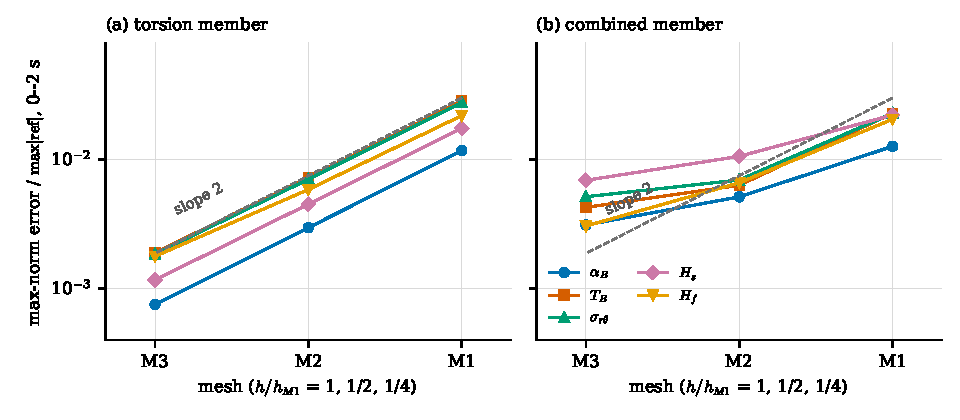
\includegraphics[width=\textwidth]{figures/rotational_convergence}
	\caption{Max-norm error of the primary rotational quantities over $0$--$2\,\mathrm{s}$ relative to $\max|\mathrm{ref}|$ against mesh size, $\Delta t=2.5\,\mathrm{ms}$: (a) torsion member, (b) combined member. The dashed line has slope two. In (b) the errors against the reference flatten (reference-error floor); a near-second-order self-difference rate is resolved sharply only for $\alpha_B$ and $H_f$, not for the torque-type quantities (Table~\ref{tab:rot_combined}). Data: \texttt{paper-data/rotational\_convergence.csv}.}
	\label{fig:rot_convergence}
\end{figure}

\emph{Nonlinear mixed terms.}
The purpose of the combined member is the interaction of the two loadings.
Defining $d_\alpha=\alpha_C-\alpha_T$, $d_T=T_{B,C}-T_{B,T}$ and $d_{\sigma_{r\theta}}$ analogously (combined minus torsion at identical mesh and settings; the reference combination is formed in the same way), these terms are $16$--$22\%$ of the combined reference maximum, i.e.\ not a small correction (the three-way radial term $u_C-u_R-u_T$ is discussed below).
Table~\ref{tab:rot_mixed} and Fig.~\ref{fig:rot_mixed} give the errors relative to the signal.
On M3 they are $1.55\%$ ($d_\alpha$), $2.47\%$ ($d_T$) and $2.19\%$ ($d_{\sigma_{r\theta}}$) over $0$--$2\,\mathrm{s}$; for $d_{\sigma_{r\theta}}$ the value is $3.4\%$ over $0$--$1.8\,\mathrm{s}$ (the window must be quoted), and the corresponding $d_T$ value is $2.6\%$.
The decrease with mesh is monotone but slow (observed orders $0.2$--$1.4$ over both windows), and the terms are reproduced to $1.5$--$2.5\%$ of their size, not converged to the reference.
The terms are resolved on their own: the bound obtained if the errors of the combined and torsion runs were uncorrelated is $0.025$, $0.037$ and $0.033$ of the signal on M3 for $d_\alpha$, $d_T$ and $d_{\sigma_{r\theta}}$ over $0$--$2\,\mathrm{s}$ (over $0$--$1.8\,\mathrm{s}$: $0.025$, $0.039$ and $0.048$), so that none of the three relies on error cancellation.
The number of non-orthogonal correctors has no effect on them (M2 values with 0 and 2 correctors are identical); halving $\Delta t$ moves $d_T$ by $0.6\%$ and $d_{\sigma_{r\theta}}$ by $0.4\%$ of the signal ($d_\alpha$ by $0.014\%$), and the absolute tolerance on M2 by $3.5\times10^{-5}$ ($d_\alpha$), $5.4\times10^{-3}$ ($d_T$) and $4.0\times10^{-3}$ ($d_{\sigma_{r\theta}}$; $6.2\times10^{-3}$ over $0$--$1.8\,\mathrm{s}$) of the signal, dominated by the torque and traction noise; the corresponding noise allowance (combined-run noise propagated to the signal) is $7.9\times10^{-3}$ for $d_T$ and $5.6\times10^{-3}$ for $d_{\sigma_{r\theta}}$ over $0$--$2\,\mathrm{s}$ ($8.8\times10^{-3}$ and $8.6\times10^{-3}$ over $0$--$1.8\,\mathrm{s}$), i.e.\ a sizeable fraction of the reproduced errors of $2.2$--$3.4\%$.

\begin{table}[htbp]
	\centering
	\small
	\setlength{\tabcolsep}{4pt}
	\caption{Mixed-term error as a percentage of the signal, $0$--$2\,\mathrm{s}$ (last row: $d_{\sigma_{r\theta}}$ over $0$--$1.8\,\mathrm{s}$), and observed orders. Signal: maximum of the reference mixed term; $d_T$ is a torque per radian of interface rotation and per metre of depth (full-annulus torque per metre of depth: $2\pi$ times larger, $468\,\mathrm{N\,m/m}$); $\sigma_{r\theta}$ in Pa. Source: \texttt{paper-data/rotational\_mixed\_terms.csv} }
	\label{tab:rot_mixed}
	\begin{tabular}{llrrrrr}
		\toprule
		Term & Signal & M1 & M2 & M3 & $p_{12}$ & $p_{23}$ \\
		\midrule
		$d_\alpha$ & $1.81\times10^{-2}$\,rad & 2.22 & 1.80 & 1.55 & 0.30 & 0.22 \\
		$d_T$ & 74.4\,N\,m\,m$^{-1}$\,rad$^{-1}$ & 8.09 & 3.85 & 2.47 & 1.07 & 0.64 \\
		$d_{\sigma_{r\theta}}$ & 90.3\,Pa & 7.17 & 3.12 & 2.19 & 1.20 & 0.51 \\
		$d_{\sigma_{r\theta}}$, $0$--$1.8\,\mathrm{s}$ & 58.7\,Pa & 10.17 & 3.95 & 3.36 & 1.37 & 0.23 \\
		\bottomrule
	\end{tabular}
\end{table}

\begin{figure}[htbp]
	\centering
	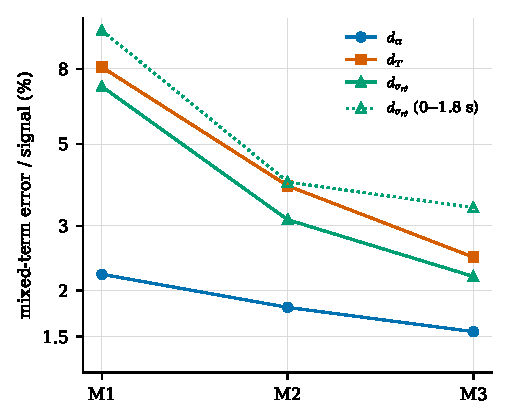
\includegraphics[width=0.55\textwidth]{figures/rotational_mixed_terms}
	\caption{Error of the nonlinear mixed terms relative to their signal on the three meshes: $0$--$2\,\mathrm{s}$ (solid) and, for $d_{\sigma_{r\theta}}$, $0$--$1.8\,\mathrm{s}$ (dotted). Data: \texttt{paper-data/rotational\_mixed\_terms.csv}.}
	\label{fig:rot_mixed}
\end{figure}

\emph{Radial member.}
The radial-only verification is incomplete and is not part of the evidence above.
At the verification setting only M1 completed; M2 stalled at $t=0.11\,\mathrm{s}$ (IQN-ILS stagnation at the coupling tolerance, not an instability), and M3 was not run.
The three-way radial interaction term $u_C-u_R-u_T$ was evaluated on M1 only (error $26\%$ of its signal, uncorrected bound far above one) and is \emph{not verified}.

\paragraph{Lesson.}
The case separates what a rotational FSI benchmark can show cleanly from what it cannot.
Rotation, torque, shear traction and angular momentum of the torsion member converge at observed orders close to two against a reference that is resolved far below the CFD error.
The combined member shows that nominal self-convergence of the CFD solutions (resolved sharply only for $\alpha_B$ and $H_f$) need not imply convergence to the reference: a reference-error floor, only partly traced to a known wall-traction effect, appears at a level a torsion-only test would not reveal; it is visible in the individual rotational quantities of the combined member (Table~\ref{tab:rot_combined}) as well as in the mixed terms, and is restricted to the quantities named there.
Finally, the finest mesh could not be run to $2\,\mathrm{s}$ with \texttt{nNonOrthogonalCorrectors}~0: the fluid outer iteration lost contractivity near $1.81\,\mathrm{s}$, which the coarser meshes did not show. Two non-orthogonal correctors removed this (halving $\Delta t$ also did), and no unique root cause is established.

\paragraph{Limitations and status.}
\begin{itemize}
	\item The reference is a reduced, planar, rotationally invariant ($n=0$) semi-analytical model verified as described above; no second, independent nonlinear implementation has checked it. The stability of $n\neq0$ modes under FSI is neither part of the reference nor tested by the evidence reported here.
	\item Orders are observed from three meshes at one time step; asymptotic convergence is not established and no temporal order is claimed. The temporal error is $5$--$25\%$ of the M3 torsion error, and an M3 temporal estimate is not available.
	\item Max-norm torque and shear-traction errors contain numerical noise of $\approx2.4\times10^{-4}$ (torsion) and $\approx1.3\times10^{-3}$ (combined) of the maximum, which makes the observed and self-difference orders of these quantities uncertain (torsion M2--M3 half-widths $\pm0.18$--$0.31$; combined self-difference intervals up to $\pm0.75$, so that the self-orders of $T_B$, $\sigma_{r\theta}$ and $T_A$ are noise-limited); the absolute-tolerance difference between M3 and M1/M2 is bounded on M2 only.
	\item The normal-traction quantities ($u_B$, $\sigma_{rr}$, $p_b$) are excluded from order claims; the combined reference-error floor ($\approx2.5$--$5.2\times10^{-3}$, for $\alpha_B$, $T_B$, $\sigma_{r\theta}$, $T_A$ and $H_f$ only; $H_s$, $w$, $KE_s$ and $P$ lie above it) is only partly explained and the roughly one-third contribution of the viscous normal-stress transmission is not a proven unique mechanism; the radial family is incomplete at the verification setting (M1 only; M2 stalled at $t=0.11\,\mathrm{s}$; M3 not run) and $u_C-u_R-u_T$ is not verified; consecutive-save ALE/GCL checks were not possible.
	\item With \texttt{nNonOrthogonalCorrectors}~0 the M3 torsion run loses fluid-iteration contractivity near $1.81\,\mathrm{s}$; the root cause is not identified.
	\item Items missing for category A (proposed): member-specific self-convergence studies of the CFD solutions to the reference limit, a pinned reproducibility kit and an explicit ``planar, rotationally invariant ($n=0$) branch'' statement in the case documentation; the combined member is not category A while the floor origin is open.
	\item In the start-up ramp ($0.0275$--$0.0325\,\mathrm{s}$) three steps of every run with $P_0\neq0$ have 51 pressure solves that stop at the iteration cap of 1000 at a residual floor proportional to $|p_b|$ ($\le10^{-13}$ of its maximum at those times); the effect on the reported quantities is immaterial (documented in the audit, not eliminated).
\end{itemize}

\paragraph{Cost and reproducibility.}
The runs below were made with OpenFOAM-v2512 and solids4foam commit \texttt{1576edcc4} on a workstation under WSL2: wall times of the accepted runs torsion M1 $90.2\,\mathrm{s}$, M2 $328.4\,\mathrm{s}$ (serial), M3 $807.7\,\mathrm{s}$ on four MPI ranks; combined M1 $98.6\,\mathrm{s}$, M2 $408.4\,\mathrm{s}$ (serial), M3 $1\,178.4\,\mathrm{s}$ on four MPI ranks (rounded to $0.1\,\mathrm{s}$).
The three-mesh torsion study therefore takes about 20 minutes run sequentially, comparable with the other core cases (Table~\ref{tab:cost}).
The case is to be contributed to solids4foam as the tutorial \texttt{tutorials/fluidSolidInteraction/radialTorsionalRing}, together with the reference script and a verification driver; the tutorial is under preparation.
The derived data behind Tables~\ref{tab:rot_torsion}--\ref{tab:rot_mixed} are in \texttt{paper-data/rotational\_*.csv}; the reference code and the case files are to be archived with a persistent identifier.

\paragraph{Relation to existing analytical FSI solutions.}
Radial and rotational fluid--solid solutions have so far been given separately: \citet{WangPironneau2026} treat a radially moving linear-elastic disc and, in a separate problem, a rotating incompressible neo-Hookean annulus with a fixed interface; \citet{Serino2019} give a radial elastic piston and a rotating elastic disk with a linear solid at small amplitude; and the analytic solutions of \citet{Hessenthaler2020} concern axial shear without radial motion.
We know of no published solution of the simultaneous finite-amplitude radial and azimuthal motion with a moving interface (in the sources we accessed; this is an absence of evidence only).
Azimuthal shear of compressible nonlinearly elastic circular tubes has been analysed by \citet{Polignone1994}.
